\chapter{Project part 1}
\section{Tasks}
\begin{enumerate}
\item Download the reference genome and the zip file with the fastq reads
\label{itm:1.1}

\item Install BWA on your computer
\label{itm:1.2}

\item Use BWA to align the Illumina reads on the reference genome
\label{itm:1.3}

\item Install IGV on your computer
\label{itm:1.4}

\item Process the sam file obtained by the BWA analysis to make a bam file
\label{itm:1.5}

\item Sort and index the bam file (see \filef{unix.pdf})
\label{itm:1.6}

\item Visualize the coverage and mate pairs on the IGV
\label{itm:1.7}

\item Manually find and comment any ``anomalous'' pair of mates
\label{itm:1.8}
\end{enumerate}

\section{Solution for task~\hyperref[itm:1.1]{1}}
I went to the Moodle of the course and downloaded the folder with the files of
the project available at this URL 
\url{https://elearning.unipd.it/math/mod/folder/view.php?id=7480}, extracting
them into a folder

\section{Solution for task~\hyperref[itm:1.2]{2}}
In order to install BWA, I run the command:
\lstinputlisting[language=bash]{res/terminal/out1.sh}

\section{Solution for task~\hyperref[itm:1.3]{3}}
In order to align the Illumina reads on the reference genome first I run the
command (in the same folder of the \filef{Lactobacillus\_casei\_genome.fasta}
file):
\lstinputlisting[language=bash]{res/terminal/out2.sh}
That index the reference genome, using the default parameters.\\
The output was:
\lstinputlisting[language=bash]{res/terminal/out3.sh}
Then I run the command:
\lstinputlisting[language=bash]{res/terminal/out4.sh}
That performs the alignment.\\
This took quite a long time and the output was quite long\footnote{It is
reported in the appendix~\ref{app:bwamem}}.
\lstinputlisting[language=bash]{res/terminal/out5.sh}
At the end of this process, the alignments are stored in the \filef{res.sam}
file.

\section{Solution for task~\hyperref[itm:1.4]{4}}
In order to install IGV I run the command:
\lstinputlisting[language=bash]{res/terminal/out6.sh}

\section{Solution for task~\hyperref[itm:1.5]{5}}
In order to process the sam file obtained by the BWA analysis to make a bam
file, I used \texttt{samtools}. First, I installed it running:
\lstinputlisting[language=bash]{res/terminal/out7.sh}
Then, I run the command:
\lstinputlisting[language=bash]{res/terminal/out8.sh}
This command will produce \filef{lact.bam} starting from the \filef{res.sam}
file. The option \texttt{-bS} is used to specify that we want as output a 
\texttt{bam} file starting from a \texttt{sam} file as input.

\section{Solution for task~\hyperref[itm:1.6]{6}}
In order to sort and index the \texttt{bam} file, first I run:
\lstinputlisting[language=bash]{res/terminal/out9.sh}
This command sort the alignments by genomic position, saving the result in the\\
\filef{lact\_sorted.bam} file. After that I run:
\lstinputlisting[language=bash]{res/terminal/out10.sh}
That produced a \filef{lact\_sorted.bam.bai} file that allow a fast random
access to the bam file.

\section{Solution for task~\hyperref[itm:1.7]{7}}
To load the genome on IGV and visualize coverage and mate pairs, after opening 
IGV I clicked on \textit{genomes} and then \textit{Load genome from file},
selecting the \filef{Lactobacillus\_casei\_genome.fasta} file. Then I loaded
the \filef{lact\_sorted.bam} file clicking on \textit{File} and then 
\textit{Load from file...} .
\begin{figure}[H]
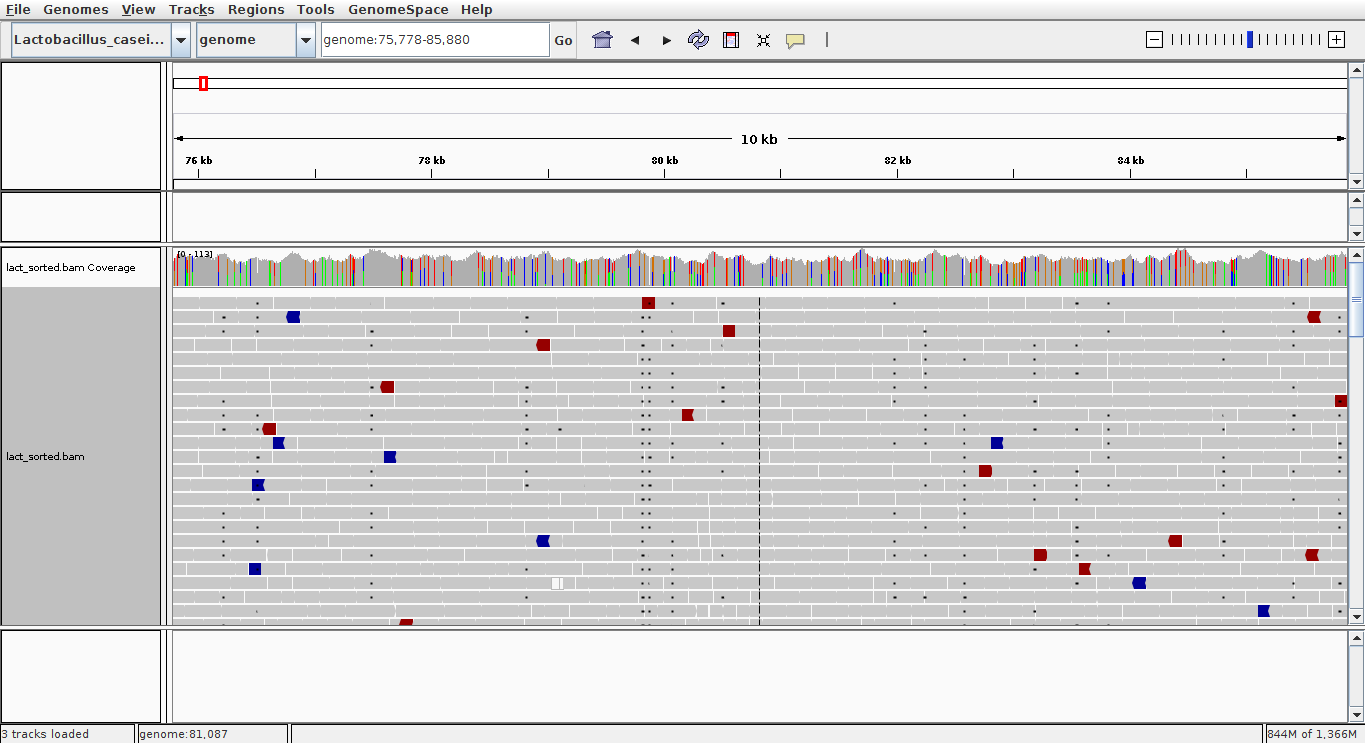
\includegraphics[scale=0.3]{point7}
\caption{IGV with the genome loaded}
\end{figure}
According to IGV documentation\footnote{
\url{https://software.broadinstitute.org/software/igv/interpreting_insert_size}}
red reads suggest possible deletion, instead blue reads means that could be
present an insertion.

\section{Solution for task~\hyperref[itm:1.8]{8}}
In this section I present some possible ``anomalies'' found in the genome
browsing it using IGV. In order to make simpler to identify them I loaded in
the program even some of the \filef{wig} files of part~\hyperref[chp:part2]{2}.
In figure~\ref{fig:longdel} we could probably see a long deletion, instead in
figure~\ref{fig:smalldel} we could probably see a small one.
\begin{figure}[H]
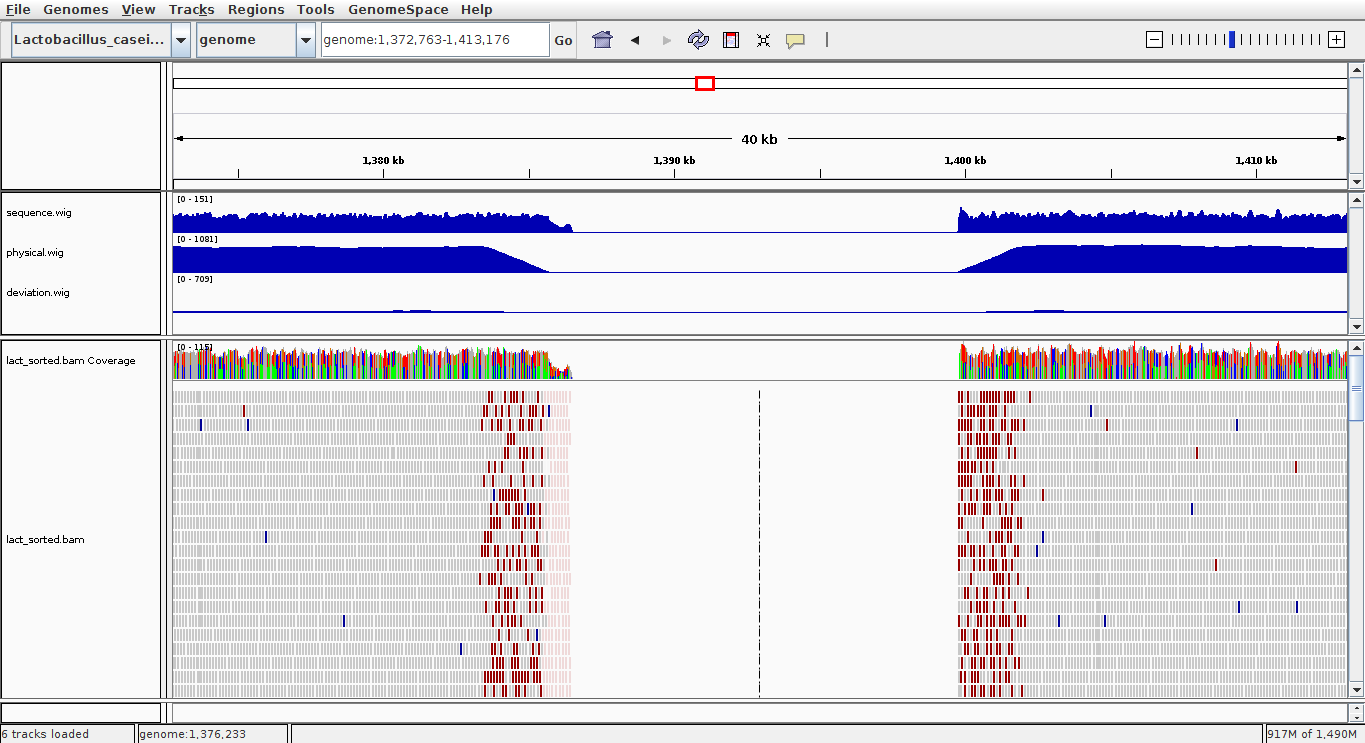
\includegraphics[scale=0.3]{long_deletion}
\caption{Long deletion}
\label{fig:longdel}
\end{figure}

\begin{figure}[H]
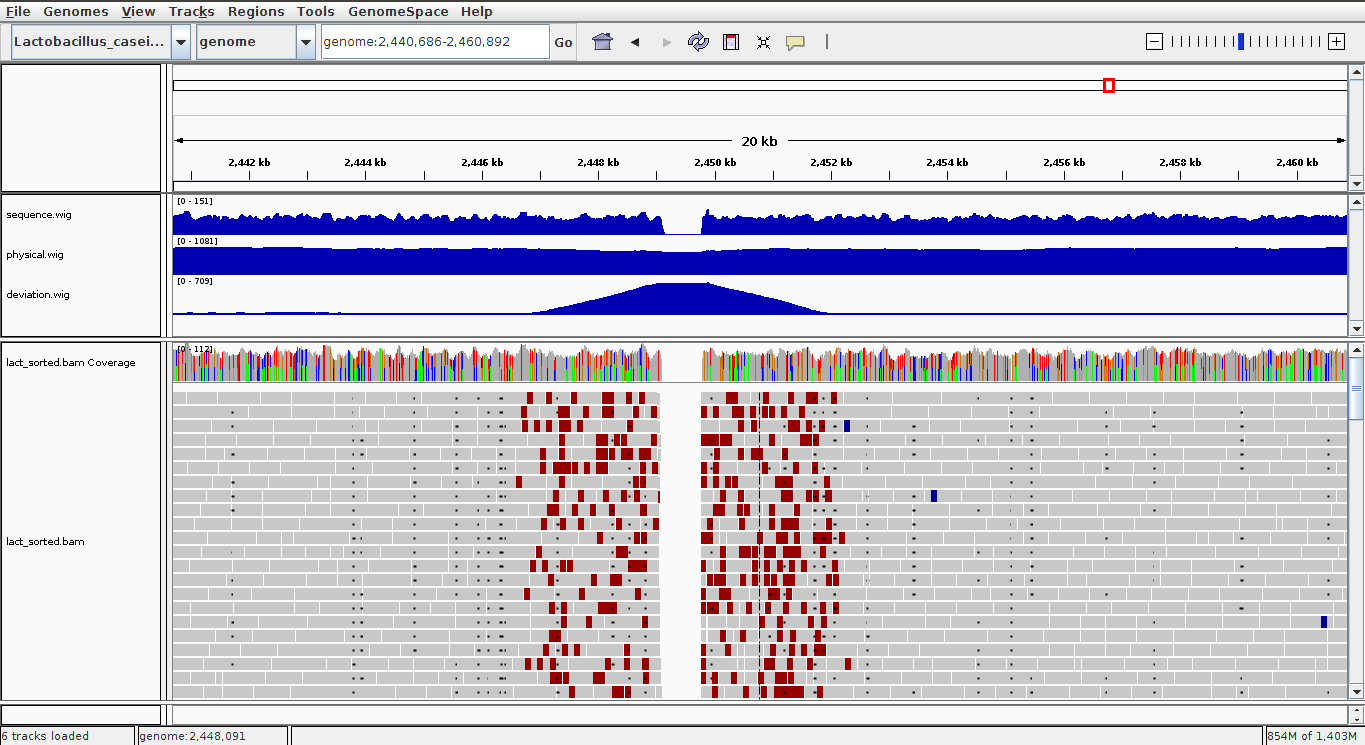
\includegraphics[scale=0.3]{small_deletion}
\caption{Small deletion}
\label{fig:smalldel}
\end{figure}

In figure~\ref{fig:longins} we could probably see a long insertion, instead in
figure~\ref{fig:smallins} we could probably see a small one.
\begin{figure}[H]
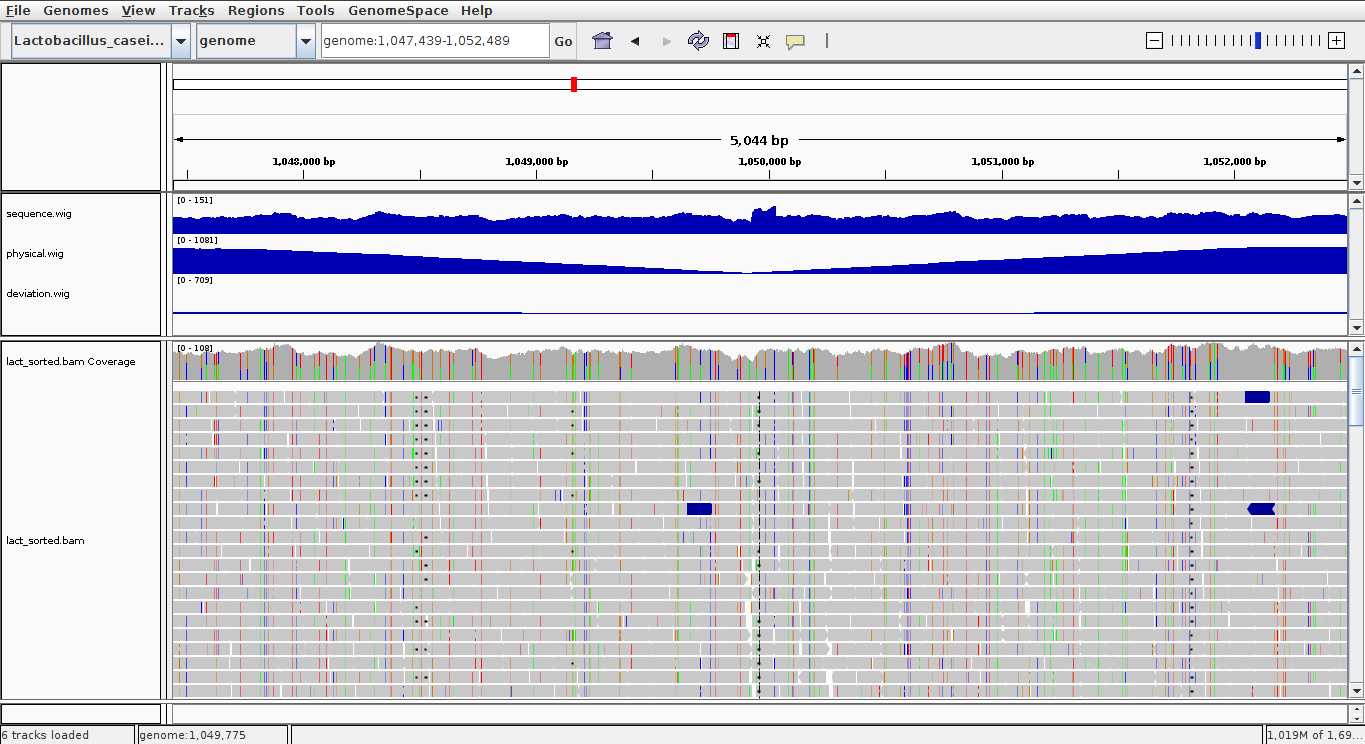
\includegraphics[scale=0.3]{long_insertion}
\caption{Long insertion}
\label{fig:longins}
\end{figure}

\begin{figure}[H]
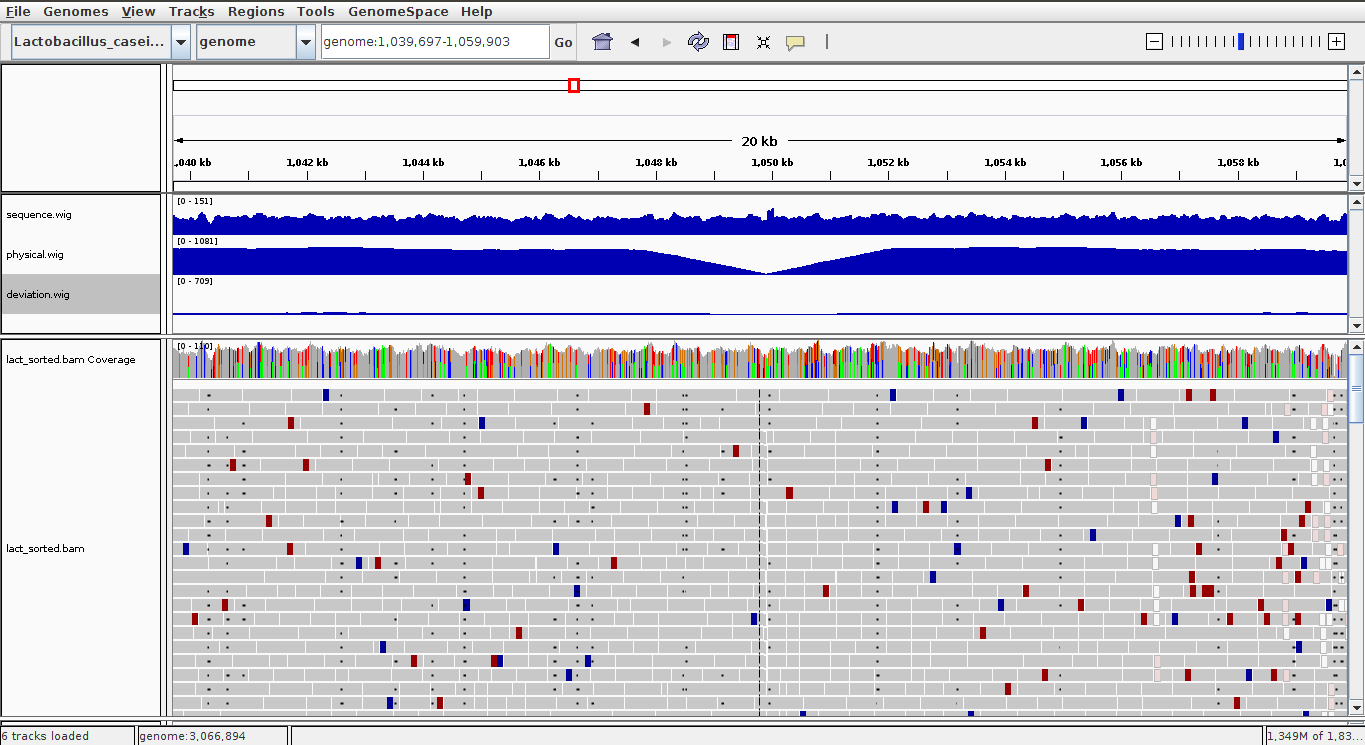
\includegraphics[scale=0.3]{small_insertion}
\caption{Small insertion}
\label{fig:smallins}
\end{figure}